% !TeX spellcheck = en_GB
% !TeX program = lualatex
%
% v 2.3  Feb 2019   Volker RW Schaa
%		# changes in the collaboration therefore updated file "jacow-collaboration.tex"
%		# all References with DOIs have their period/full stop before the DOI (after pp. or year)
%		# in the author/affiliation block all ZIP codes in square brackets removed as it was not %         understood as optional parameter and ZIP codes had bin put in brackets
%       # References to the current IPAC are changed to "IPAC'19, Melbourne, Australia"
%       # font for ‘url’ style changed to ‘newtxtt’ as it is easier to distinguish "O" and "0"
%
\documentclass[a4paper,
               %boxit,        % check whether paper is inside correct margins
               %titlepage,    % separate title page
               %refpage       % separate references
               %biblatex,     % biblatex is used
               %keeplastbox,   % flushend option: not to un-indent last line in References
               %nospread,     % flushend option: do not fill with whitespace to balance columns
               %hyphens,      % allow \url to hyphenate at "-" (hyphens)
               %xetex,        % use XeLaTeX to process the file
               %luatex,       % use LuaLaTeX to process the file
               ]{jacow}
%
% ONLY FOR \footnote in table/tabular
%
\usepackage{pdfpages,multirow,ragged2e} %
%
% CHANGE SEQUENCE OF GRAPHICS EXTENSION TO BE EMBEDDED
% ----------------------------------------------------
% test for XeTeX where the sequence is by default eps-> pdf, jpg, png, pdf, ...
%    and the JACoW template provides JACpic2v3.eps and JACpic2v3.jpg which
%    might generates errors, therefore PNG and JPG first
%
\makeatletter%
	\ifboolexpr{bool{xetex}}
	 {\renewcommand{\Gin@extensions}{.pdf,%
	                    .png,.jpg,.bmp,.pict,.tif,.psd,.mac,.sga,.tga,.gif,%
	                    .eps,.ps,%
	                    }}{}
\makeatother

% CHECK FOR XeTeX/LuaTeX BEFORE DEFINING AN INPUT ENCODING
% --------------------------------------------------------
%   utf8  is default for XeTeX/LuaTeX
%   utf8  in LaTeX only realises a small portion of codes
%
\ifboolexpr{bool{xetex} or bool{luatex}} % test for XeTeX/LuaTeX
 {}                                      % input encoding is utf8 by default
 {\usepackage[utf8]{inputenc}}           % switch to utf8

\usepackage[USenglish]{babel}

\usepackage[acronym]{glossaries}

\newglossaryentry{ptbl}{
    name={PTBL},
    description={periodic transient beam loading},
    first={periodic transient beam loading (\glsentrytext{ptbl})}
}
\newglossaryentry{hc}
{
    name={HC},
    description={harmonic cavity},
    first={harmonic cavity (\glsentrytext{hc})},
    plural={HCs},
    descriptionplural={harmonic cavities},
    firstplural={Harmonic cavities (\glsentryplural{hc})}
}
\newglossaryentry{lmci}{
    name={LMCI},
    description={longitudinal mode-coupling instability},
    first={longitudinal mode-coupling instability (\glsentrytext{lmci})}
}
%
% if BibLaTeX is used
%
\ifboolexpr{bool{jacowbiblatex}}%
 {%
  \addbibresource{jacow-test.bib}
  \addbibresource{biblatex-examples.bib}
 }{}
\listfiles

%%
%%   Lengths for the spaces in the title
%%   \setlength\titleblockstartskip{..}  %before title, default 3pt
%%   \setlength\titleblockmiddleskip{..} %between title + author, default 1em
%%   \setlength\titleblockendskip{..}    %afterauthor, default 1em

\begin{document}

\title{Slow longitudinal mode 1 instability in electron storage rings with harmonic cavities}

\author{M. B. Alves\thanks{murilo.alves@lnls.br}\textsuperscript{1}, F. H. de Sá, Brazilian Synchrotron Light Laboratory, LNLS, Campinas, Brazil\\
		\textsuperscript{1}also at Gleb Wataghin Institute of Physics, University of Campinas, UNICAMP, Campinas, Brazil}
\maketitle

%
\begin{abstract}
Recent studies have investigated a longitudinal instability that may develop in electron storage rings featuring higher-harmonic cavities. The instability, also referred to as~\gls{ptbl}, manifests as a slow oscillation of bunch longitudinal profiles following a coupled-bunch mode 1 pattern. In this contribution, we applied a well-established theory of longitudinal mode-coupling to assess the thresholds for this instability. Results obtained through this semi-analytical approach, considering different storage ring and harmonic cavity parameters, were validated using macroparticle tracking and compared against other methods proposed in previous investigations.
\end{abstract}
\section{Introduction}
\glspl{hc} are used in electron storage rings aiming to increase bunch length by adjusting longitudinal focusing. In 4\textsuperscript{th} generation synchrotron light sources, the pursuit of ultralow emittance leads to intense intrabunch Coulomb interactions, which reduce Touschek lifetime and increase beam blow-up due to intrabeam scattering. \glspl{hc} can operate passively, with its voltage generated through beam-induced wakefields. Proper tuning of the resonant frequency is crucial for coupling with beam harmonics to achieve the desired voltage. However, the \gls{hc} impedance, essential for lengthening the equilibrium bunch, can adversely affect beam stability.

Recent investigations studied mode 1 instability through theory~\cite{Venturini2018, He2022b}, simulations~\cite{He2022a}, and experiments~\cite{Cullinan2024}. Various prediction methods have been proposed, analyzing the phenomenon's dependencies on \gls{hc} and ring parameters. Referred to as~\glsfirst{ptbl} due to its slow oscillation, the instability has been accurately predicted within specific contexts. However, the accuracy of these methods is not always reproduced with different parameters and when compared to experimental data~\cite{Cullinan2024}.

The present contribution reports new findings for mode 1 instability based on simulation studies. Macroparticle tracking using MAX IV parameters was initially used to replicate the instability and explore its behavior. Then, a linear theory of \gls{lmci} for Gaussian bunches was applied to predict instability growth rates. The results were benchmarked against tested methods. Finally, we discuss how the \gls{lmci} approach can provide a new understanding of mode 1 instability phenomenology.

\section{Macroparticle tracking}
A two-dimensional longitudinal tracking was implemented in Python3~\cite{CollectiveEffectsRepo}. The code tracks the time evolution of longitudinal dynamic variables of several macroparticles in each rf bucket, in the presence of resonator wakefields and accounting for radiation damping and quantum excitation.

We tested a condition where the mode-1 instability is expected: parameters for MAX IV \SI{3}{\giga\electronvolt} storage ring, 3 passive \glspl{hc} at flat potential (\SI{300}{\milli\ampere}, main rf voltage~\SI{1.397}{\mega\volt}, \gls{hc} voltage~\SI{0.448}{\mega\volt})~\cite{Cullinan2024}. The results for oscillating bunch centroids and lengths are presented in Fig.~\ref{fig:1}.\begin{figure}[!ht]
    \centering
    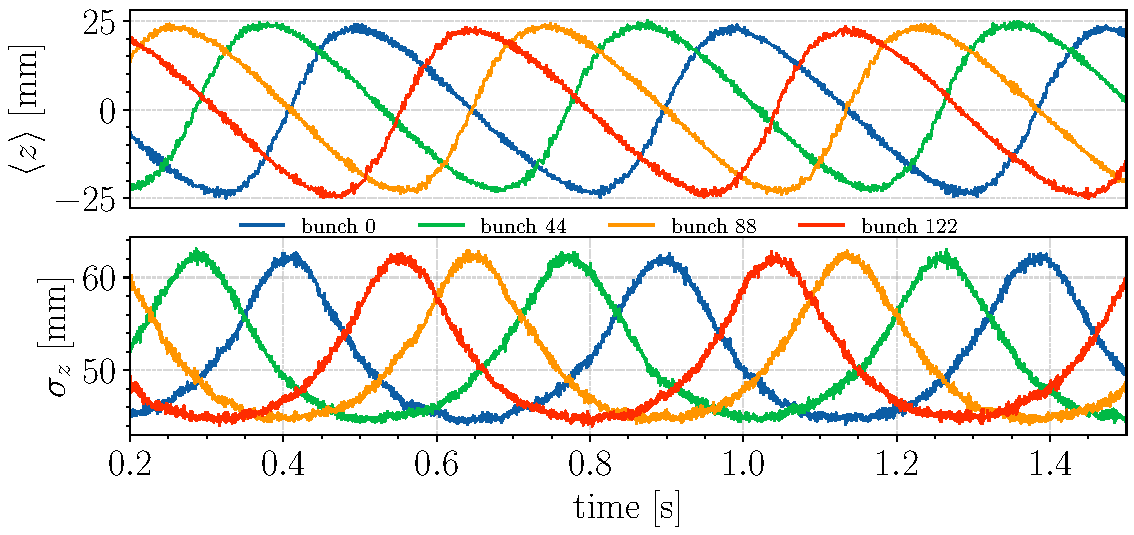
\includegraphics[width=0.48\textwidth]{MOPS32_f1.pdf}
    \caption{Mode 1 instability obtained with macroparticle tracking for MAX IV \SI{3}{\giga\electronvolt} ring and \glspl{hc} on flat potential condition. Oscillation period is about~\SI{0.5}{\second}. Simulation setup:~\num{10000} macroparticles per bunch,~\num{1.5} million turns.}
    \label{fig:1}
\end{figure}

The modal analysis of the oscillation shows that the coupled-bunch mode 1 is the most unstable mode, oscillating with a low frequency of~\SI{2}{\hertz}.

We investigated the dependence of the instability on the number of macroparticles per bunch. The goal was to understand if details of the bunch profiles and sampling of the distorted potential-well are essential features to the instability. We ran tracking simulations with increasing values of \gls{hc} voltages with 50 and only 1 macroparticle per bunch (point bunch in this case). Interestingly, the behavior of oscillation amplitudes with respect to \gls{hc} voltage is essentially independent of the number of particles, and the most unstable mode is always mode 1 for both cases, as presented in Figure~\ref{fig:2}.\begin{figure}
    \centering
    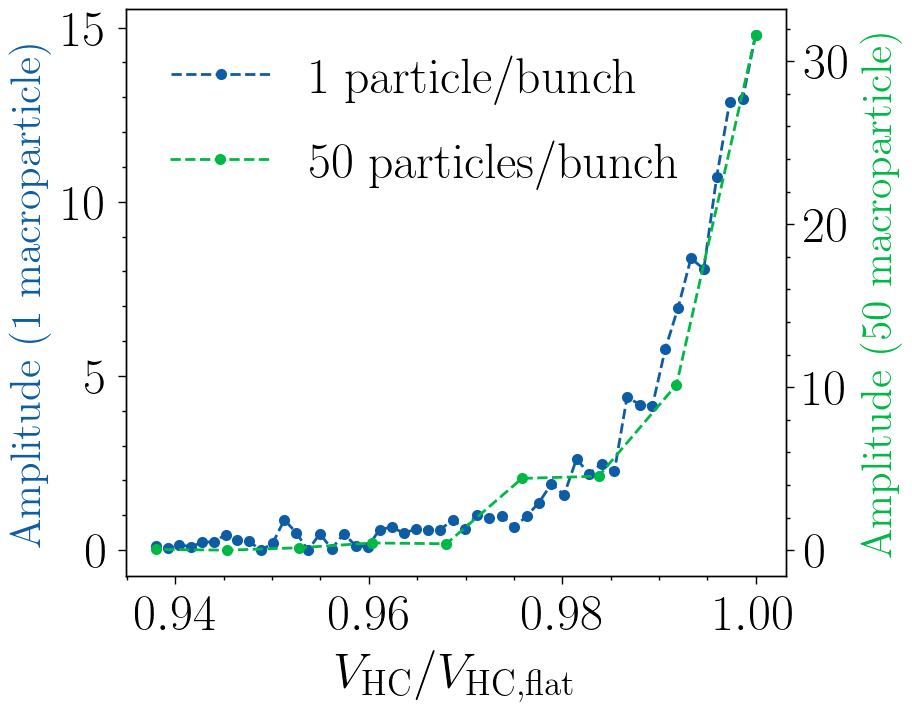
\includegraphics[width=0.24\textwidth]{MOPS32_f2a.png}
    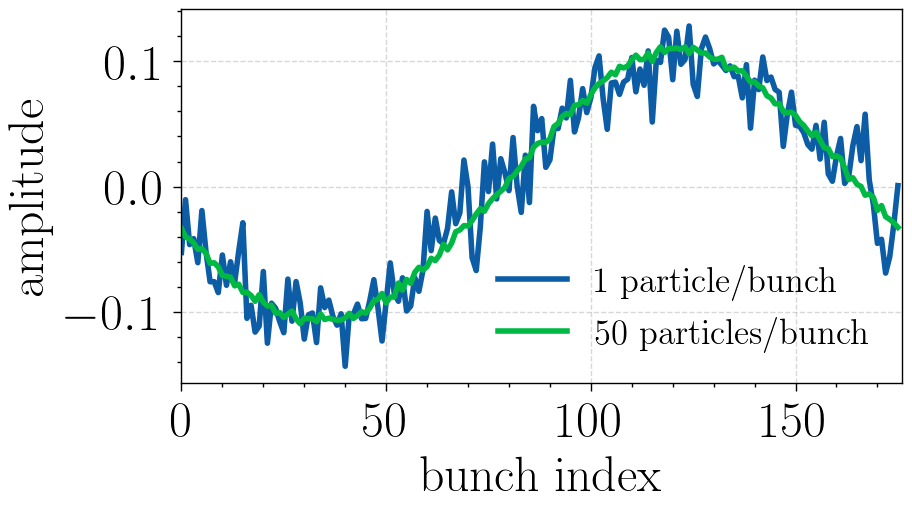
\includegraphics[width=0.24\textwidth]{MOPS32_f2b.png}
    \caption{Left: Mode 1 oscillation amplitude for 1 and 50 macroparticles per bunch as a function of harmonic voltage. Right: signature of the most unstable mode.}
    \label{fig:2}
\end{figure}

These tests with macroparticle tracking suggest two main aspects of the mode 1 instability: only the motion of bunch centroids (point bunch approximation) should capture the underlying instability mechanism, and the nonlinearities within the bunch (intrabunch Landau damping) should be negligible. Another important observation is that the variations in bunch length are only a consequence of the instability, due to variations in the potential well-distortion introduced by the oscillating bunch centroids.

% Another important observation is that, even when the instability is driven only by dipole motion, the variations in bunch length are consequence of the oscillation of bunch centroids in double-rf systems, where significant wake-induced voltages on passive \glspl{hc} are created by the beam.
% \section{Longitudinal mode coupling instability (\gls{lmci})}
\section{Vlasov solver}
We investigated the mode 1 instability employing Suzuki's frequency-domain solution of Vlasov equation for longitudinal instabilities, which allows mode coupling between different azimuthal and radial modes of the bunch motion~\cite{Suzuki1983}. The theory assumes that the single-particle dynamics is linear and that the longitudinal bunch distribution is Gaussian. This makes the theory suitable for studying instabilities in single-rf systems, neglecting potential-well distortion. Nevertheless, the findings from macroparticle tracking motivated us to use this Gaussian linear theory to study the mode~1 instability in \gls{hc} systems.

Suzuki's solution yields the infinite matrix equation~\cite{Suzuki1983}:
% \begin{equation}
%     \frac{m - \lambda}{m} a_{k^\prime}^{(m)} = -i \frac{e I_0\alpha}{2\pi \nu_s^2 E \sigma_\theta^2} \sum_{m^\prime=-\infty}^{\infty} \sum_{k = 0}^{\infty} M_{m^\prime k}^{m k^\prime} a_k^{(m^\prime)}
% \end{equation}
\begin{align}
\left(\frac{\Omega}{\omega_s}\right)^2 b_{k}^{(m)} &= \sum_{m^\prime=1}^{\infty} \sum_{k^\prime = 0}^{\infty} A_{m^\prime k^\prime}^{m k} b_{k^\prime}^{(m^\prime)}, \\
    A_{m^\prime k^\prime}^{m k} &= m^2 \delta_{m^\prime m}\delta_{k^\prime k} + i \frac{m^2 ec^2 \alpha I_0}{\pi \sigma_z^2 \omega_s^2 E}  M_{m^\prime k^\prime}^{m k},
\end{align}
where $(m, m^\prime)$ and $(k, k^\prime)$ are indices for the azimuthal and radial modes, respectively. $\alpha$ is the momentum compaction factor, $\sigma_z$ the bunch length, $\omega_s$ the angular synchrotron frequency, $E$ the ring energy, $c$ the speed of light and $e>0$ the elementary charge. A uniform filling with total current $I_0$ is assumed. The coupling matrix depends on the longitudinal impedance~$Z_{\parallel}$ and beam spectrum
\begin{equation}
   M_{m^\prime k^\prime}^{m k} = \sum_{p=-\infty}^{\infty} \frac{Z_{\parallel}(\omega_p)}{\omega_p} i^{m^\prime-m} I_{m^\prime k^\prime}\left(\frac{\omega_p}{\omega_0}\right) I_{m k}\left(\frac{\omega_p}{\omega_0}\right),
\end{equation}
where $\omega_p = (ph + \mu)\omega_0 + \Omega$, $\omega_0$ is the angular revolution frequency, $h$ the harmonic number and $\mu$ the coupled-bunch mode. For Gaussian bunches, the functions $I_{m k}(p)$ have the analytic form:
\begin{align}
    I_{m k}(p) &= \frac{1}{\sqrt{(m+k)!k!}} \left(\frac{\zeta_p}{2}\right)^{m+2k} \exp\left({-\frac{\zeta_p^2}{4}}\right),\\\zeta_p &= \sqrt{2}\sigma_z \omega_p/c. \nonumber
\end{align}
To solve the matrix problem, the sums are truncated to $m_\mathrm{max}$ and $k_\mathrm{max}$. Moreover, the approximation $\Omega \approx \omega_s$ is applied to the finite coupling matrix $M_{m^\prime k^\prime}^{m k}$. The analysis can be specialized to mode 1 by the evaluation of coupling matrix at~$\omega_p \approx (ph + 1 + \nu_s)\omega_0$. Then the coherent frequencies are obtained by diagonalization. $\mathrm{Re}(\Omega)\slash 2\pi$ is the coherent frequency of oscillation and $\mathrm{Im}(\Omega)$ is the exponential growth rate. An instability is predicted if the growth rate surpass the radiation damping rate.

The \gls{lmci} theory was applied to the mode 1 instability in the presence of \gls{hc} fields, requiring a minor yet important adaptation in the calculation process. The values for bunch length and incoherent synchrotron frequency used in the calculation were derived from the longitudinal equilibrium of the double-rf system with \glspl{hc}. Therefore, it is essential to determine the equilibrium parameters with a self-consistent solution to Haissinki equation~\cite{AlvesSa2023} before instability calculations. With this scheme, the potential-well distortion caused by the \gls{hc} is not entirely neglected for the instability analysis, as its impact on bunch length and incoherent synchrotron frequency is accounted. However, it is important to note that this scheme disregards intrabunch nonlinearities, thus Landau damping effects are neglected. We will refer to this scheme as ``Gaussian \gls{lmci}''.

In Gaussian \gls{lmci}, the incoherent synchrotron frequency is a crucial input. For non-linear single-particle dynamics, such as with \gls{hc} fields, the frequency becomes a function of amplitude. Therefore, a constant value can only represent an effective value for the amplitude-dependent frequency. In general, it is not clear which measure is appropriate for this effective frequency. Possible options are:
\begin{subequations}
\begin{align}
    \langle\omega_s\rangle_\mathrm{quadratic} &= \alpha c \sigma_\delta / \sigma_z,\label{eq:freq_by_bunlen} \\
    \langle \omega_s \rangle_z &= \int_{-\infty}^{\infty}\mathrm{d}z~\lambda(z) \left(-\frac{\alpha hc}{2\pi E\omega_\mathrm{rf}} V^{\prime}(z)\right)^{1/2}, \label{eq:freq_by_z}\\
    \langle \omega_s \rangle_J &= 2\pi \int_{0}^{\infty}\mathrm{d}J~\Psi(J) \omega_s(J), \label{eq:freq_by_J} \\
    \langle\omega_s\rangle_\mathrm{center} &= \omega_s(J=0).\label{eq:freq_bunch_center}
\end{align}
\end{subequations}Equation~\eqref{eq:freq_by_bunlen} is satisfied for a quadratic longitudinal potential. Equation~\eqref{eq:freq_by_z} represents the local synchrotron frequency averaged by the bunch line-density $\lambda(z)$. Equation~\eqref{eq:freq_by_J} is the global synchrotron frequency over a complete synchrotron cycle averaged by the action distribution within the bunch~$\Psi(J)$. Equation~\eqref{eq:freq_bunch_center} denotes the frequency at the bunch center and also has a local character. For the cases studied, Eqs.~\eqref{eq:freq_by_bunlen} and Eq.~\eqref{eq:freq_by_z} yield similar values, while Eqs.~\eqref{eq:freq_by_J} and~\eqref{eq:freq_bunch_center} provide lower values.

For a quadratic potential, all expressions yield the same value. For a quartic potential, when there is perfect cancellation of first and second derivative of rf voltage at the synchronous phase (thus $\omega_s(0) = 0$), it can be shown that~\cite{Venturini2018, Lindberg2018}
\begin{equation}
    \langle \omega_s \rangle_\mathrm{quartic} = \frac{2\pi~2^{3/4}}{\Gamma^2(1/4)} \alpha c \sigma_\delta\sigma_z \approx 0.8039 \langle\omega_s\rangle_\mathrm{quadratic}
\end{equation}

\begin{figure*}
    \centering
    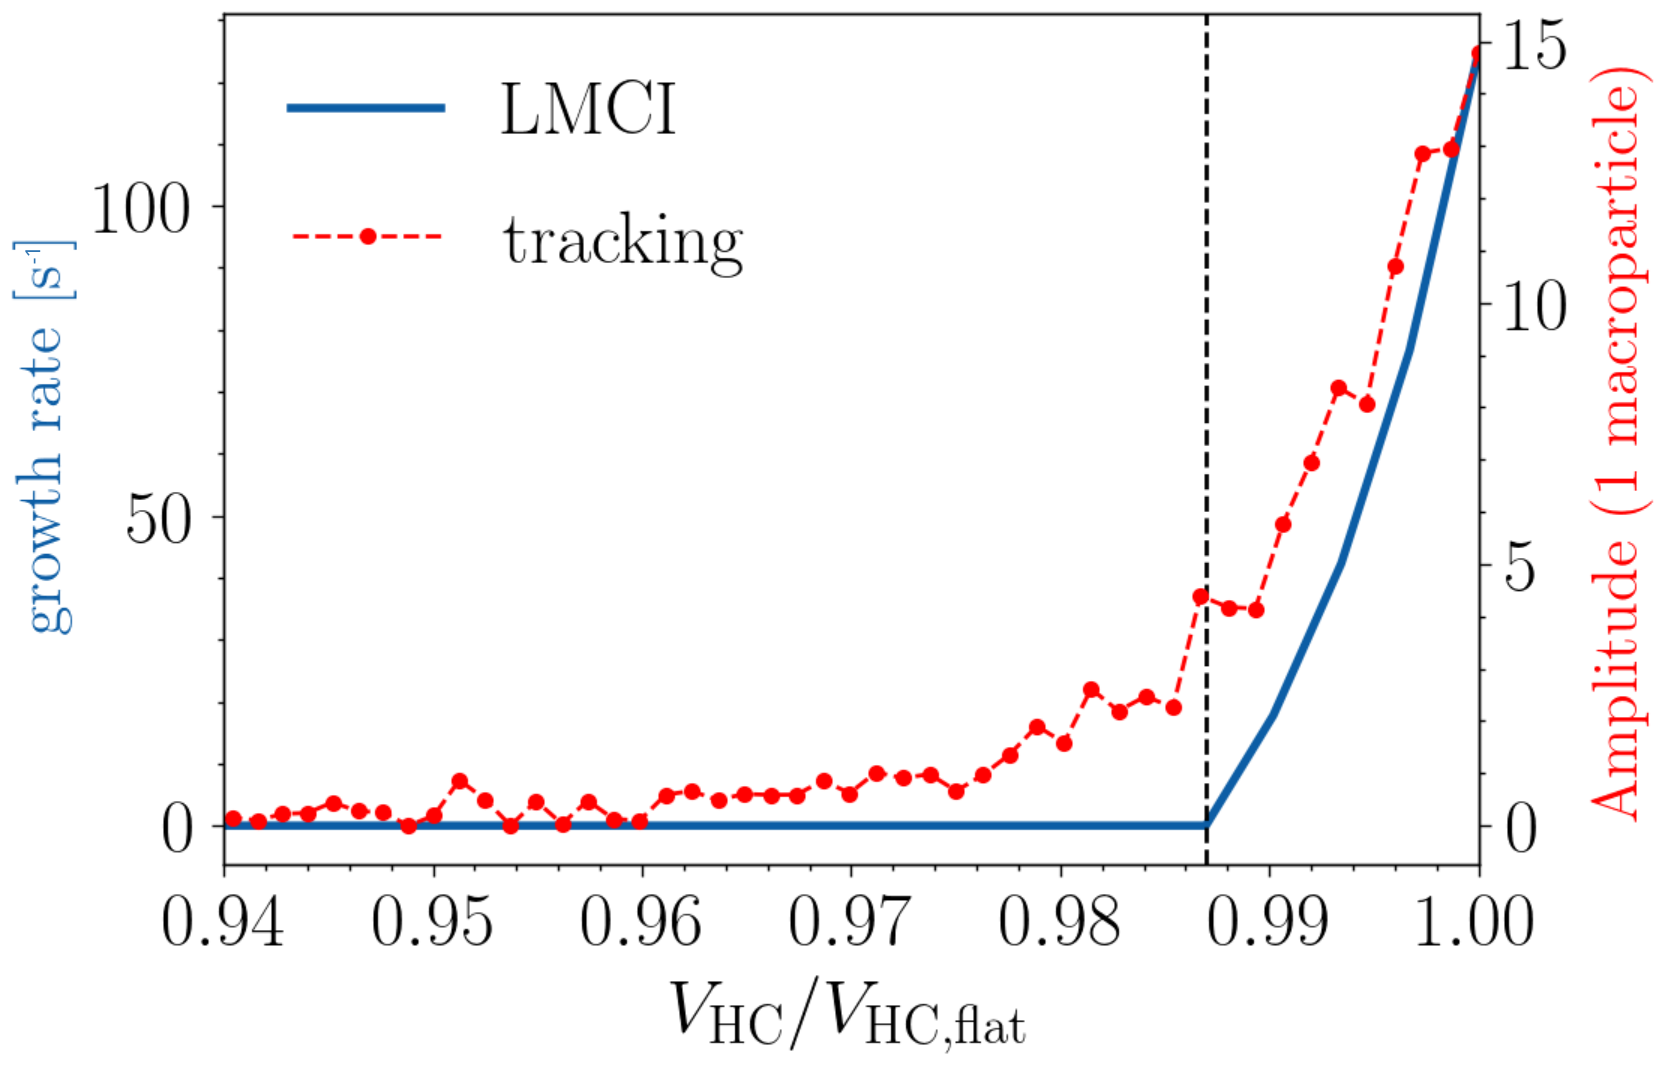
\includegraphics[width=0.35\textwidth]{MOPS32_f3a.png}
    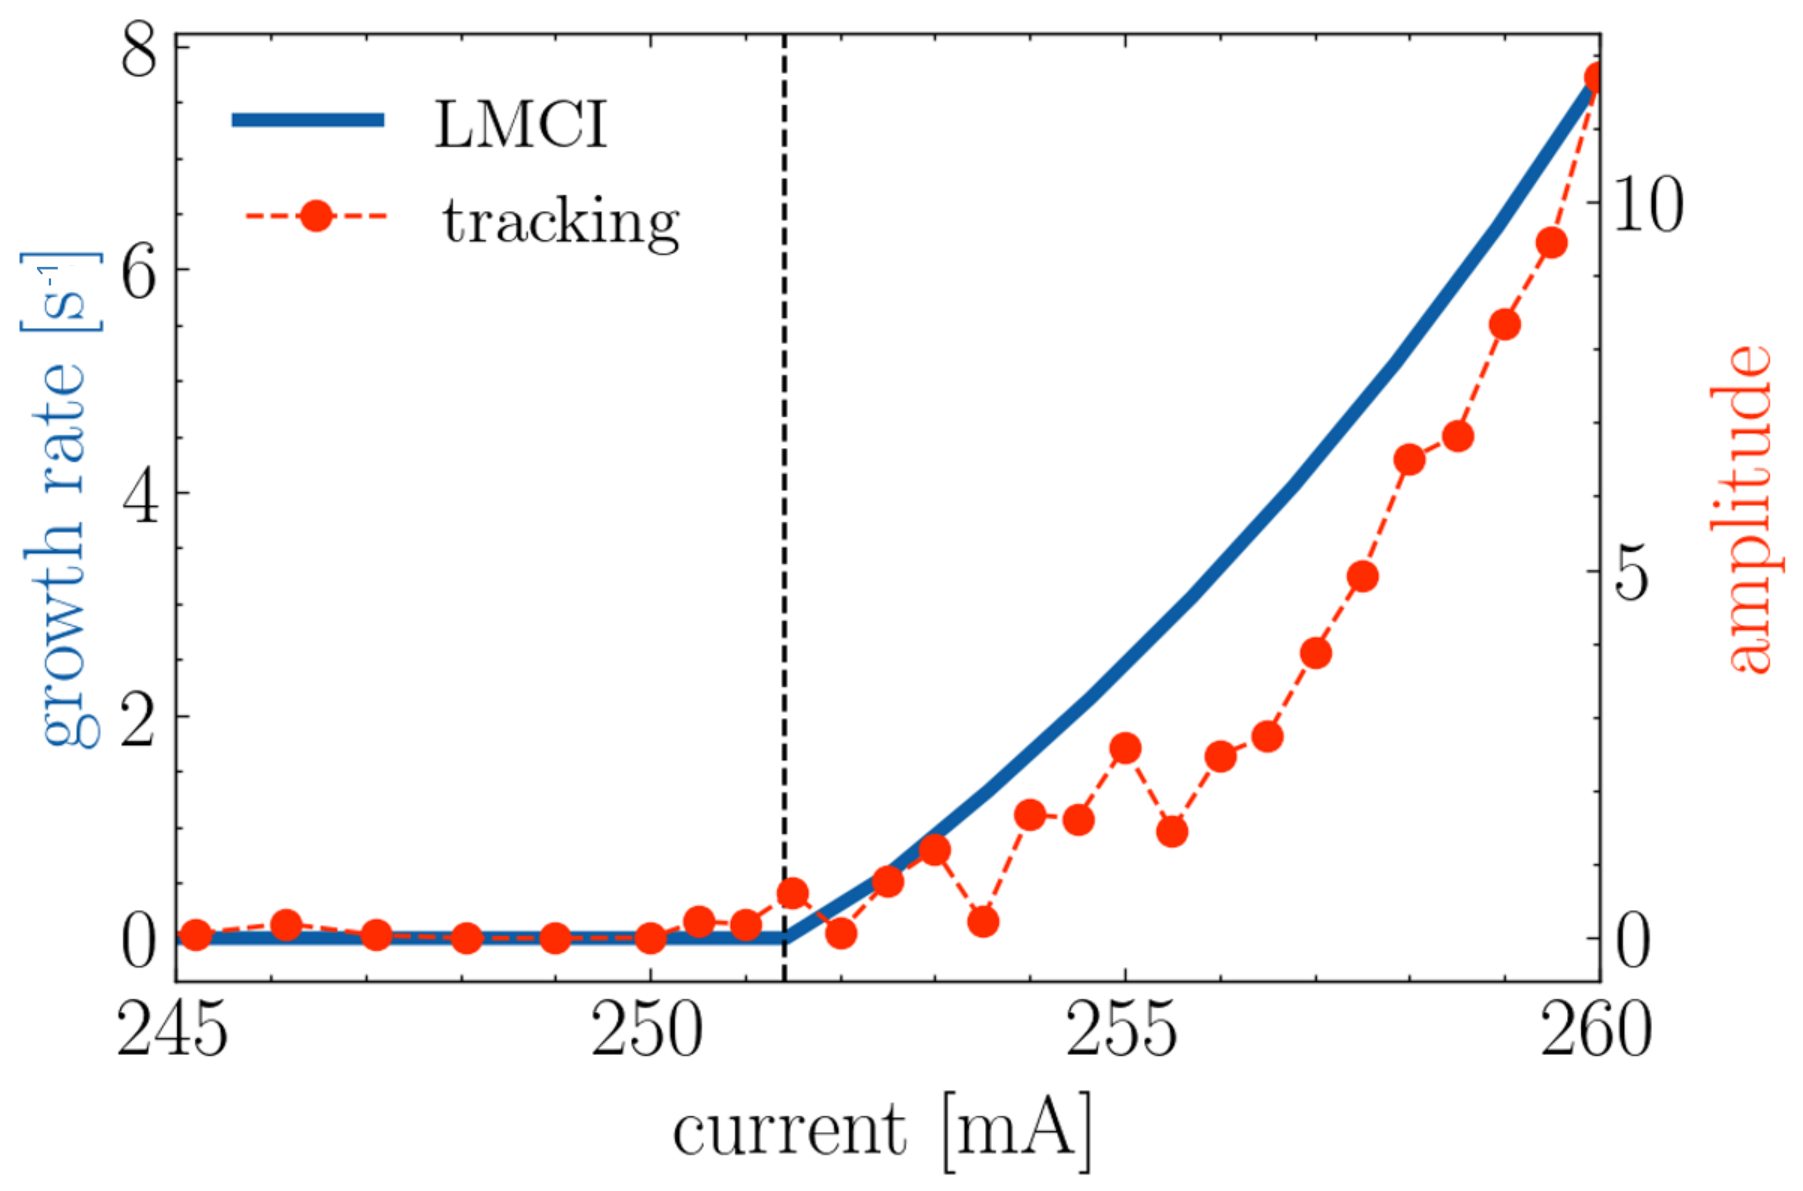
\includegraphics[width=0.34\textwidth]{MOPS32_f3b.png}
    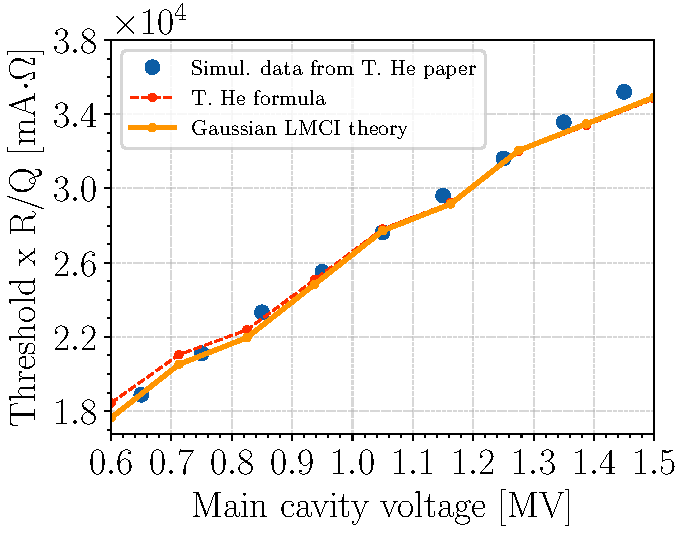
\includegraphics[width=0.30\textwidth]{MOPS32_f3c.pdf}
    \caption{Left: Harmonic voltage threshold for MAX IV storage ring. Middle: Total current threshold for HALF storage ring. Threshold obtained by \gls{lmci} is \SI{251}{\milli\ampere}. Right: The product of total current threshold and \gls{hc} $R/Q$ as a function of main rf cavity voltage for HALF storage ring. Simulated data from~\cite{He2022a}. Formula from~\cite{He2022b}.}
    \label{fig:benchmark}
\end{figure*}
\subsection{Benchmarking \gls{lmci} Results}
A series of comparisons between the growth rates calculated with \gls{lmci} theory and oscillation amplitudes from tracking simulation is presented in Fig.~\ref{fig:benchmark}. The effective incoherent synchrotron frequency used in all calculations was the equivalent quadratic potential from Eq.~\eqref{eq:freq_by_bunlen}. A convergence test was performed for the truncation parameters $m_\mathrm{max}$ and $k_\mathrm{max}$. The results already converge with $m_\mathrm{max}=2$ and $k_\mathrm{max}=1$.

For MAX IV parameters as reported in~\cite{Cullinan2024}, \SI{300}{\milli\ampere} and $V_\mathrm{rf} = \SI{1.397}{\mega\volt}$, the flat potential \gls{hc} voltage is~\SI{448}{\kilo\volt}, the threshold \gls{hc} voltage is~\SI{442}{\kilo\volt}. For HALF parameters as reported in~\cite{He2022a}, with \gls{hc} tuned to near flat potential, the calculated threshold current is \SI{251}{\milli\ampere}, while the reported value is~\SI{259}{\milli\ampere}, a difference of only~\SI{3}{\percent}. In~\cite{He2022a} it is also reported that the product of threshold current with \gls{hc}'s~$R/Q$ depends linearly on the main rf voltage. This behavior was also obtained from our calculations, showing very good agreement with independent tracking results from~\cite{He2022a} and the analytical formula from~\cite{He2022b}.

\section{Instability mechanism}
Figure~\ref{fig:6} shows the evolution of coherent modes of coupled-bunch mode 1 as the \gls{hc} voltage increases. We note that a positive growth rate is excited when a radial mode associated with $m=1$ approaches the zero frequency, when there's not enough coherent focusing to keep the modes in stable oscillations. Note that other radial mode associated with $m=1$ follows the reduction of incoherent $\omega_s$, while the coherent mode that drives the instability is additionally shifted by the imaginary (reactive) part of impedance~\cite{Alves:HarmonLIP24}. This suggests that the coherent mode is shifted out of the band of incoherent frequencies spread, then stabilization by Landau damping is not possible.

Based on this mechanism, the phenomenology reported in~\cite{He2022a, Cullinan2024} can be explained: (i) higher main rf voltage: $\omega_s$ without the \gls{hc} increases with $\sqrt{V_\mathrm{rf}}$, thus a larger coherent shift is needed to approach the zero frequency; (ii) larger \gls{hc} detuning: the \gls{hc} fields are lowered, implying in less cancellation of longitudinal focusing, thus a higher $\omega_s$ and shorter bunch; (iii) \gls{hc} $R/Q$: for high $Q$ resonators, $\mathrm{Im}(Z_\parallel) \propto R/Q$. Since $\mathrm{Re}(\Delta \Omega) \propto \mathrm{Im}(Z_\parallel)$, a larger $R/Q$ produces a larger coherent shift. Ref.~\cite{Venturini2018} first highlighted that the instability is mainly driven by the imaginary part of the impedance.

\begin{figure}
    \centering
    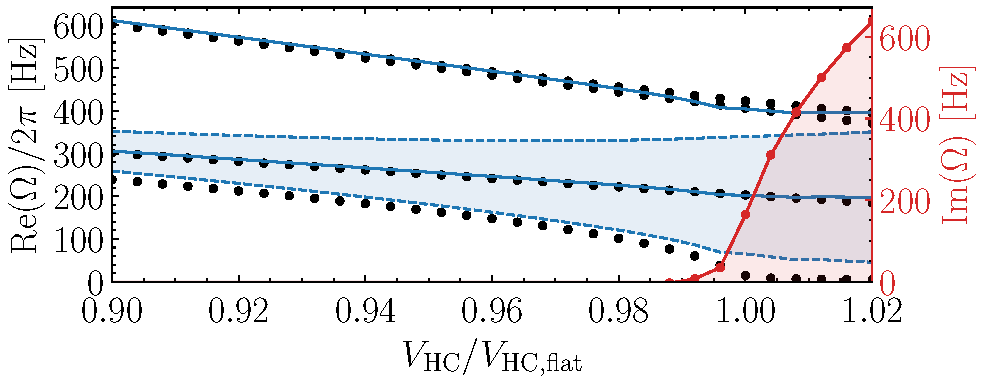
\includegraphics[width=0.48\textwidth]{MOPS32_f4.pdf}
    \caption{Coherent frequencies for coupled-bunch 1 as a function of \gls{hc} voltage for MAX IV parameters represented in black dots. Calculation made with $m_\mathrm{max}=2$ and $k_\mathrm{max}=1$. The mode $m=2$ introduces an additional shift to $m=1$ and it was needed for accurate threshold predictions. Blue solid curves are multiples of the average incoherent synchrotron frequency and the shaded blue area is the std, representing the frequency spread.}
    \label{fig:6}
\end{figure}

\section{Conclusion}
The mode 1 instability induced by \glspl{hc} in electron storage rings was investigated. The instability was reproduced with 1 macroparticle per bunch in tracking simulations and accurately predicted with a calculation scheme based on a linear theory of instabilities with longitudinal mode-coupling for Gaussian bunches slightly adapted to a \gls{hc} system. Further studies are needed to better understand which is the most appropriate measure of effective incoherent frequency for this scheme. Instability occurs when a radial mode associated to the dipole motion approaches the zero frequency. A direct conclusion is that variations of parameters that either increase the incoherent synchrotron frequency or reduce the coherent shift of coupled-bunch mode 1 helps to increase the threshold for current or \gls{hc} voltage. In 4\textsuperscript{th} generation synchrotrons, the natural synchrotron frequencies are typically low, which make new machines operating with \glspl{hc} more susceptible to the mode 1 instability.
\section{Acknowledgments}
The authors thank Liu Lin and Ximenes Resende for fruitful discussions and suggestions.
%
% only for "biblatex"
%
\ifboolexpr{bool{jacowbiblatex}}%
	{\printbibliography}%
	{%
	% "biblatex" is not used, go the "manual" way

	%\begin{thebibliography}{99}   % Use for  10-99  references
	\begin{thebibliography}{9} % Use for 1-9 references

    \bibitem{Venturini2018}
	M. Venturini, \textquotedblleft{Passive higher-harmonic rf cavities with general settings and multibunch instabilities in electron storage rings}\textquotedblright, \textit{Phys. Rev. Accel. Beams}, vol. 21, no. 11, p. 114404, Nov. 2018.\\ \url{doi:10.1103/PhysRevAccelBeams.21.114404}
	
    \bibitem{He2022b}
    T. He, \textquotedblleft{Novel perturbation method for judging the stability of the equilibrium solution in the presence of passive harmonic cavities}\textquotedblright, \textit{Phys. Rev. Accel. Beams}, vol. 25, no. 9, p. 094402, Sep. 2022.\\ \url{doi:10.1103/PhysRevAccelBeams.25.094402}

    \bibitem{He2022a}
	T. He, W. Li, Z. Bai, and L. Wang, \textquotedblleft{Periodic transient beam loading effect with passive harmonic cavities in electron storage rings}\textquotedblright, \textit{Phys. Rev. Accel. Beams}, vol. 25, no. 2, Feb. 2022.\\ \url{doi:10.1103/PhysRevAccelBeams.25.024401}
	
    \bibitem{Cullinan2024}
	F. J. Cullinan, \AA{}. Andersson, J. Breunlin, M. Brosi, and P. F. Tavares, \textquotedblleft{Experimental observation of a mode-1 instability driven by Landau cavities in a storage ring}\textquotedblright, \textit{Phys. Rev. Accel. Beams}, vol. 27, no. 4, p. 044403, Apr. 2024.\\ \url{doi:10.1103/PhysRevAccelBeams.27.044403}

    \bibitem{CollectiveEffectsRepo}
    F. H. de Sá and M. B. Alves,
    ``pycolleff and cppcolleff: Modules for impedance analysis and wake-field induced instabilities evaluation'', 2023,\\
    \url{https://doi.org/10.5281/zenodo.8088076}

    \bibitem{Suzuki1983}
    T.~Suzuki, Y.~Chin, and K.~Satoh,
    ``Mode Coupling Theory and Bunch Lengthening in {SPEAR} {II}''
    \emph{Part. Accel.} \textbf{13} (1983), 179-198,
    KEK Preprint 82-26

    \bibitem{AlvesSa2023}
	M. B. Alves and F. H. de Sá, \textquotedblleft{Equilibrium of longitudinal bunch distributions in electron storage rings with arbitrary impedance sources and generic filling patterns}\textquotedblright, \textit{Phys. Rev. Accel. Beams}, vol. 26, no. 9, p. 094402, Sep. 2023.\\ \url{doi:10.1103/PhysRevAccelBeams.26.094402}

    \bibitem{Lindberg2018}
	R. R. Lindberg, \textquotedblleft{Theory of coupled-bunch longitudinal instabilities in a storage ring for arbitrary rf potentials}\textquotedblright, \textit{Phys. Rev. Accel. Beams}, vol. 21, no. 12, p. 124402, Dec. 2018.\\ \url{doi:10.1103/PhysRevAccelBeams.21.124402}

    \bibitem{Alves:HarmonLIP24}
    M. B. Alves,
    ``Predictions of slow longitudinal mode-1 instability in storage rings with harmonic cavities''
    presented at HarmonLIP, Grenoble, France, 2024,
    \url{https://indico.esrf.fr/event/122/contributions/665/attachments/390/777/HarmonLIP2024_PredictMode1_v1.pdf}
	\end{thebibliography}
} % end \ifboolexpr

\end{document}
